% Minh họa thuật toán/trace đã khóa; không chạy retrieval hoặc model mới.
\documentclass[10pt]{article}
\usepackage[T1]{fontenc}
\usepackage{lmodern}
\usepackage[paperwidth=180mm,paperheight=190mm,margin=4mm]{geometry}
\usepackage{tikz}
\usetikzlibrary{arrows.meta}
\pagestyle{empty}
\setlength{\parindent}{0pt}
\hyphenpenalty=10000
\exhyphenpenalty=10000
\definecolor{ink}{HTML}{1F3445}
\definecolor{teal}{HTML}{126B80}
\definecolor{ochre}{HTML}{9A581D}
\begin{document}
\centering
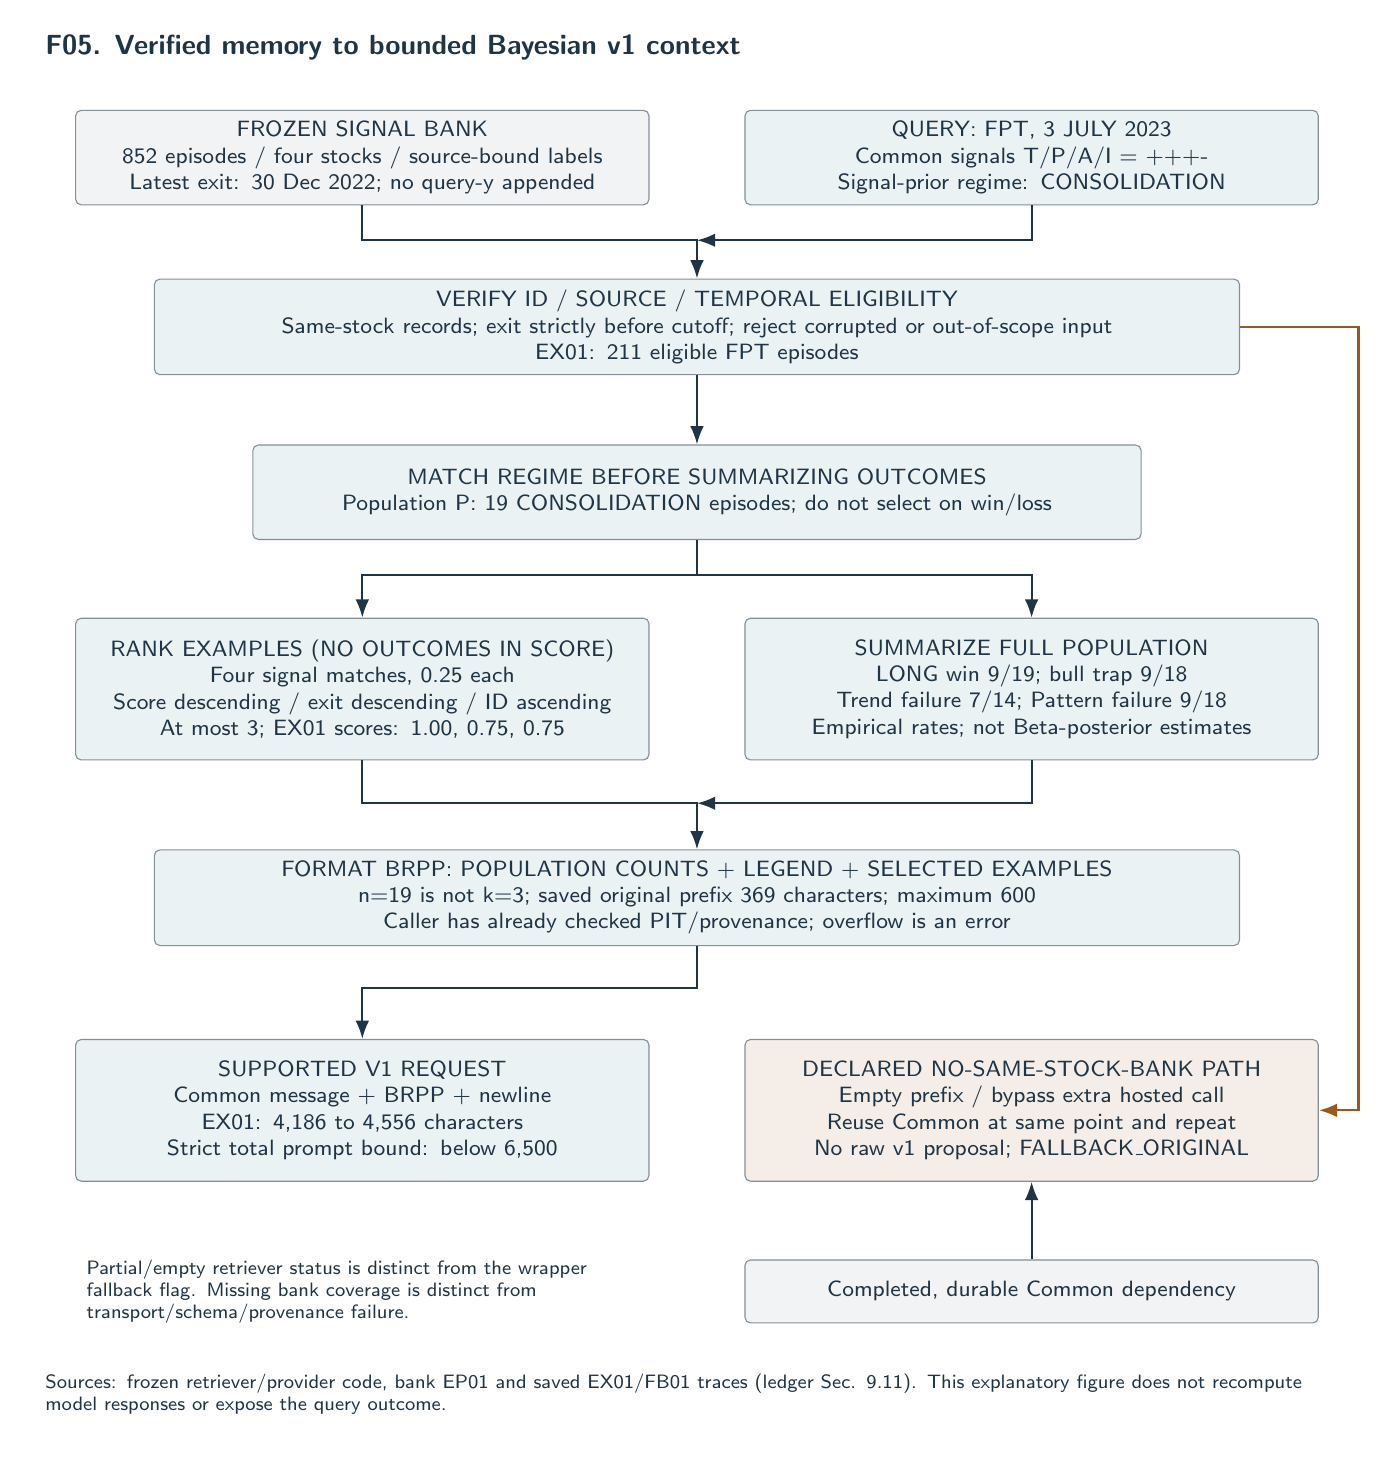
\begin{tikzpicture}[x=1cm,y=1cm,>=Latex,font=\sffamily\footnotesize,text=ink,
 box/.style={draw=ink!55,rounded corners=2pt,align=center,text width=7cm,minimum height=1.2cm,inner sep=4pt},
 flow/.style={->,thick,draw=ink}]
\path[use as bounding box] (0,0) rectangle (17.0,18.0);
\node[anchor=west,font=\sffamily\bfseries] at (.1,17.75) {F05. Verified memory to bounded Bayesian v1 context};
\node[box,fill=ink!6] (bank) at (4.25,16.35)
 {FROZEN SIGNAL BANK\\852 episodes / four stocks / source-bound labels\\Latest exit: 30 Dec 2022; no query-y appended};
\node[box,fill=teal!9] (query) at (12.75,16.35)
 {QUERY: FPT, 3 JULY 2023\\Common signals T/P/A/I = +++-\\Signal-prior regime: CONSOLIDATION};
\node[box,fill=teal!9,text width=13.5cm] (eligible) at (8.5,14.2)
 {VERIFY ID / SOURCE / TEMPORAL ELIGIBILITY\\Same-stock records; exit strictly before cutoff; reject corrupted or out-of-scope input\\EX01: 211 eligible FPT episodes};
\draw[flow] (bank.south) -- (4.25,15.3) -| (eligible.north);
\draw[flow] (query.south) -- (12.75,15.3) -- (8.5,15.3);
\node[box,fill=teal!9,text width=11cm] (population) at (8.5,12.1)
 {MATCH REGIME BEFORE SUMMARIZING OUTCOMES\\Population P: 19 CONSOLIDATION episodes; do not select on win/loss};
\draw[flow] (eligible) -- (population);
\node[box,fill=teal!9,minimum height=1.8cm] (rank) at (4.25,9.6)
 {RANK EXAMPLES (NO OUTCOMES IN SCORE)\\Four signal matches, 0.25 each\\Score descending / exit descending / ID ascending\\At most 3; EX01 scores: 1.00, 0.75, 0.75};
\node[box,fill=teal!9,minimum height=1.8cm] (stats) at (12.75,9.6)
 {SUMMARIZE FULL POPULATION\\LONG win 9/19; bull trap 9/18\\Trend failure 7/14; Pattern failure 9/18\\Empirical rates; not Beta-posterior estimates};
\draw[flow] (population.south) -- (8.5,11.05) -| (rank.north);
\draw[flow] (8.5,11.05) -| (stats.north);
\node[box,fill=teal!9,text width=13.5cm] (prefix) at (8.5,6.95)
 {FORMAT BRPP: POPULATION COUNTS + LEGEND + SELECTED EXAMPLES\\n=19 is not k=3; saved original prefix 369 characters; maximum 600\\Caller has already checked PIT/provenance; overflow is an error};
\draw[flow] (rank.south) -- (4.25,8.15) -- (8.5,8.15) -- (prefix.north);
\draw[flow] (stats.south) -- (12.75,8.15) -- (8.5,8.15);
\node[box,fill=teal!9,minimum height=1.8cm] (decision) at (4.25,4.25)
 {SUPPORTED V1 REQUEST\\Common message + BRPP + newline\\EX01: 4,186 to 4,556 characters\\Strict total prompt bound: below 6,500};
\draw[flow] (prefix.south) -- (8.5,5.8) -| (decision.north);
\node[box,fill=ochre!10,minimum height=1.8cm] (bypass) at (12.75,4.25)
 {DECLARED NO-SAME-STOCK-BANK PATH\\Empty prefix / bypass extra hosted call\\Reuse Common at same point and repeat\\No raw v1 proposal; FALLBACK\_ORIGINAL};
\draw[flow,draw=ochre] (eligible.east) -- (16.9,14.2) -- (16.9,4.25) -- (bypass.east);
\node[box,fill=ink!6,minimum height=.8cm] (common) at (12.75,1.95)
 {Completed, durable Common dependency};
\draw[flow] (common) -- (bypass);
\node[align=left,text width=7.0cm,font=\sffamily\scriptsize] at (4.25,1.95)
 {\raggedright Partial/empty retriever status is distinct from the wrapper fallback flag.
 Missing bank coverage is distinct from transport/schema/provenance failure.\par};
\node[anchor=west,align=left,text width=16.7cm,font=\sffamily\scriptsize] at (.1,.65)
 {Sources: frozen retriever/provider code, bank EP01 and saved EX01/FB01 traces (ledger Sec. 9.11).
 This explanatory figure does not recompute model responses or expose the query outcome.};
\end{tikzpicture}
\end{document}
